\chapter{Improving the Model}

\section{Weighted Loss}

One of the biggest problems highlighted above is low recall on less common qualities. Two common methods for dealing with long-tailed distributions are re-sampling and weighting the loss function.~\citet{CurriculumLearning} also explore the use of curriculum learning as form of re-sampling which we do not explore here. Sampling is explored by~\citet{BalanceRandomForestACR} but they use a different model based on pre-computing chroma vectors and re-sampling these chroma vectors for use in training a random forest for frame-wise decoding. In our setting, re-sampling training patches of audio may be interesting but is left as future work as it would require significant effort to manage sampling many chords at once. Weighting has been explored by~\citet{ACRLargeVocab1} however their weighting is over chord classes and chord `components' which they define in their work. We employ a similar but simpler implementation here.

TODO: Cite Reweighting vs Resampling and claim it won't make a big difference.

A standard method of weighting is to multiply the loss function by the inverse of the given class' frequency, with a parameter controlling the strength of the weighting. This is defined as below.

\begin{equation}
    w_c = \frac{1}{(\text{count}(c) + 1)^\alpha}
\end{equation}

Where $w_c$ is the weight for chord $c$, $\text{count}(i)$ is the number of frames with chord $c$ in the dataset and $\alpha$ is a hyperparameter controlling the strength of weighting. $\alpha=0$ results in no weighting and increasing $alpha$ increases the severity of weighting. We add $1$ in the denominator to avoid dividing by $0$ and to diminish the effect of chords with very few occurrences. We then define normalised weights $w_c^*$ below.

\begin{equation}\label{eq:weighted_loss}
    w_c^* = \frac{w_c}{s} \text{ where } s = \frac{\sum_{c\in \mathcal{C}} \text{count}(c)\cdot w_c}{\sum_{c\in \mathcal{C}} \text{count}(c)}
\end{equation}

Where $\mathcal{C}$ is the set of all chords in the vocabulary. This keeps the expected weight at $1$ such that the effective learning rate remains the same. We calculate these values over the training set. We test values of $\alpha$ in the set \{0, 0.05, 0.1, \ldots, 0.95, 1\}. The plot in Figure~\ref{fig:weighted_loss} shows the effect of the weighting on the model's performance.

\begin{figure}[H]
    \centering
    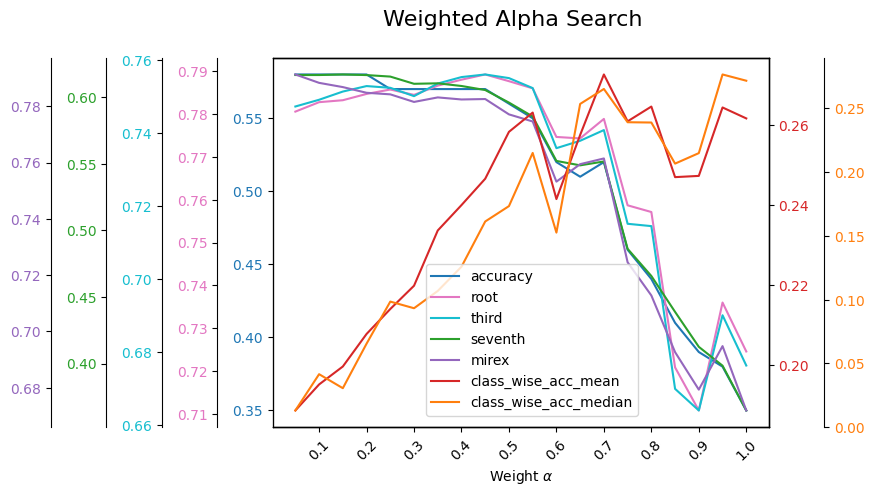
\includegraphics[width=1.0\textwidth]{figures/weight_alpha_search.png}
    \caption{Effect of weighted loss on the \emph{CRNN} model with varying $\alpha$. As we increase $\alpha$, class-wise metrics improve but accuracy-based metrics worsen. We claim a sweet-spot in the middle where we trade only a little overall performance for better class-wise recall. We choose this to be $\alpha = 0.55$. The \texttt{root} and \texttt{third} metrics improve and less than $3\%$ is lost on other metrics while mean class-wise accuracy improves by $6\%$ and the median improved by $0.2$. This plot also reveals strong correlation between metrics. }\label{fig:weighted_loss}
\end{figure}

\section{Decoding}\label{sec:decoding}

As observed in~\ref{sec:smoothness}, taking the maximum probability over each frame results in $170$ transitions per song as opposed to the $104$ seen in the ground truth data. We implemented a decoding step over the frame-wise probability vectors to smooth predicted labels. Common choices for decoding models include a conditional random field (CRF)~\citep{ACRLargeVocab1, BTC} and a hidden Markov model (HMM)~\citep{BalanceRandomForestACR}. 

For the sake of simplicity, we first implemented an HMM and found it to be able to smooth chords predictions well. The HMM treats the frame-wise probabilities as emission probabilities and the chord labels as hidden states.~\citet{CQTvsChroma} note that using a transition matrix with all non-recurrent transitions equally likely performs similarly to using a learned transition matrix. We adopt such a transition matrix for our HMM, with a parameter $\beta$ denoting the self-transition probabilities, and all other transition probabilities equal to $\frac{1-\beta}{C-1}$. We then compute a forward and backward pass of the Viterbi algorithm to output the most likely sequence of chords.

A plot of the effect of $\beta$ on the model's performance and the number of transitions per song is shown in Figure~\ref{fig:hmm_beta_search}. From this plot we conclude that smoothing has little affect on \texttt{root} while successfully reducing the number of transitions per song to that of the true labels. We choose $\beta = 0.2$ as it results in $102$ transitions per song while maintaining high performance.

\begin{figure}[H]
    \centering
    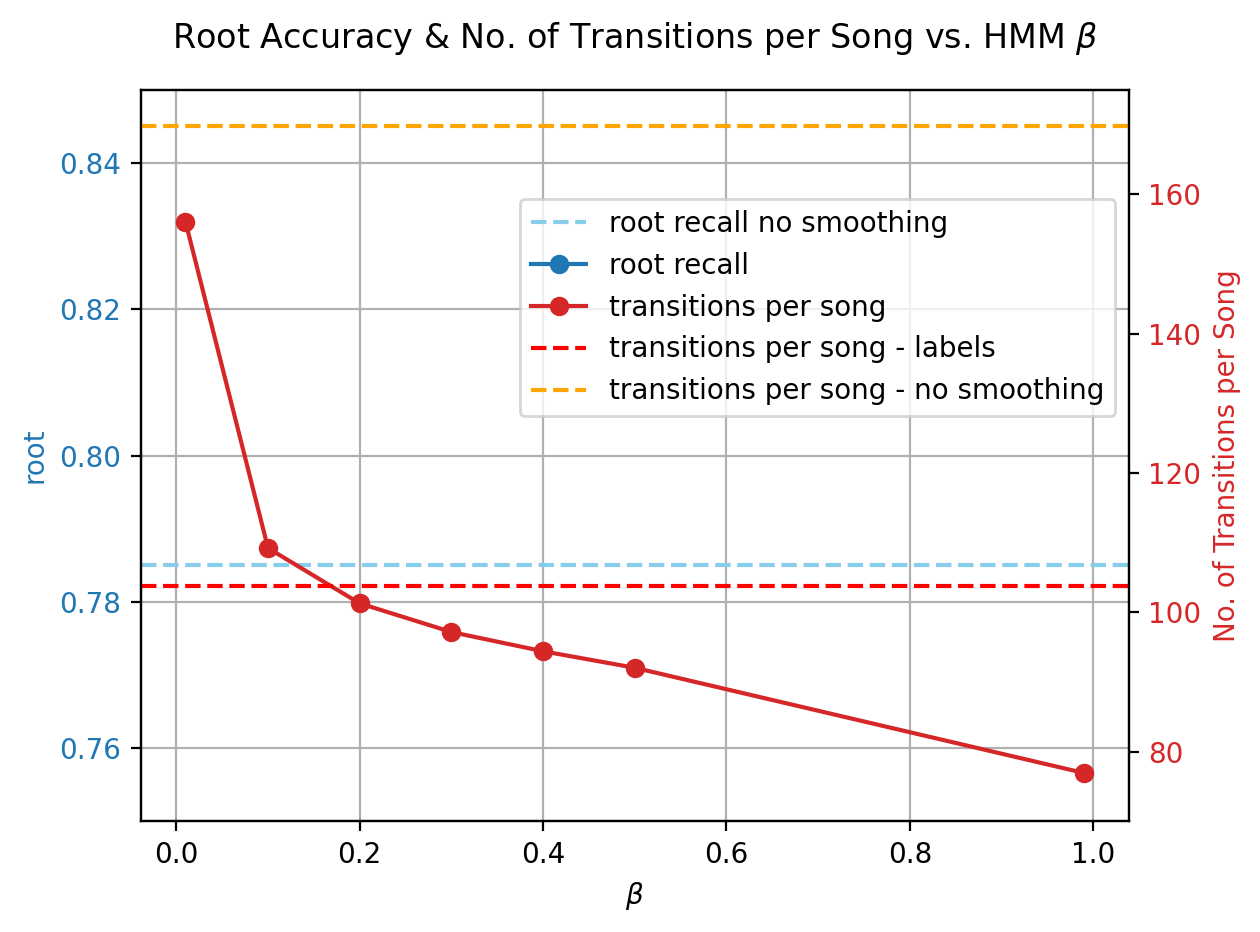
\includegraphics[width=0.8\textwidth]{figures/hmm_beta_vs_root_transitions.png}
    \caption{Effect of the HMM smoothing parameter $\beta$ on the \emph{CRNN} model. As we increase $\beta$, the number of transitions per song decreases. We choose $\beta = 0.2$ as it results $102$ transitions per song, very close to the $104$ of the ground truth. Performance is stable across $\beta$ with a slight degradation for $\beta > 0.3$. Other performance metrics showed similarly stable results. }\label{fig:hmm_beta_search}
\end{figure}

The effect of the HMM on the incorrect regions previously discussed in Section~\ref{sec:smoothness} can be found in Appendix~\ref{app:histogram_over_region_lengths}. The HMM reduced the percentage of incorrect regions which are a single frame long from $26.7\%$ to $16.7\%$. A more intuitive way to see the effect of the HMM is to look at a section of a song which was the model previously predicted many chord transitions for. We show this in Figure~\ref{fig:hmm_smoothing_example}.

\begin{figure}[H]
    \centering
    \hspace{-1.5cm}
    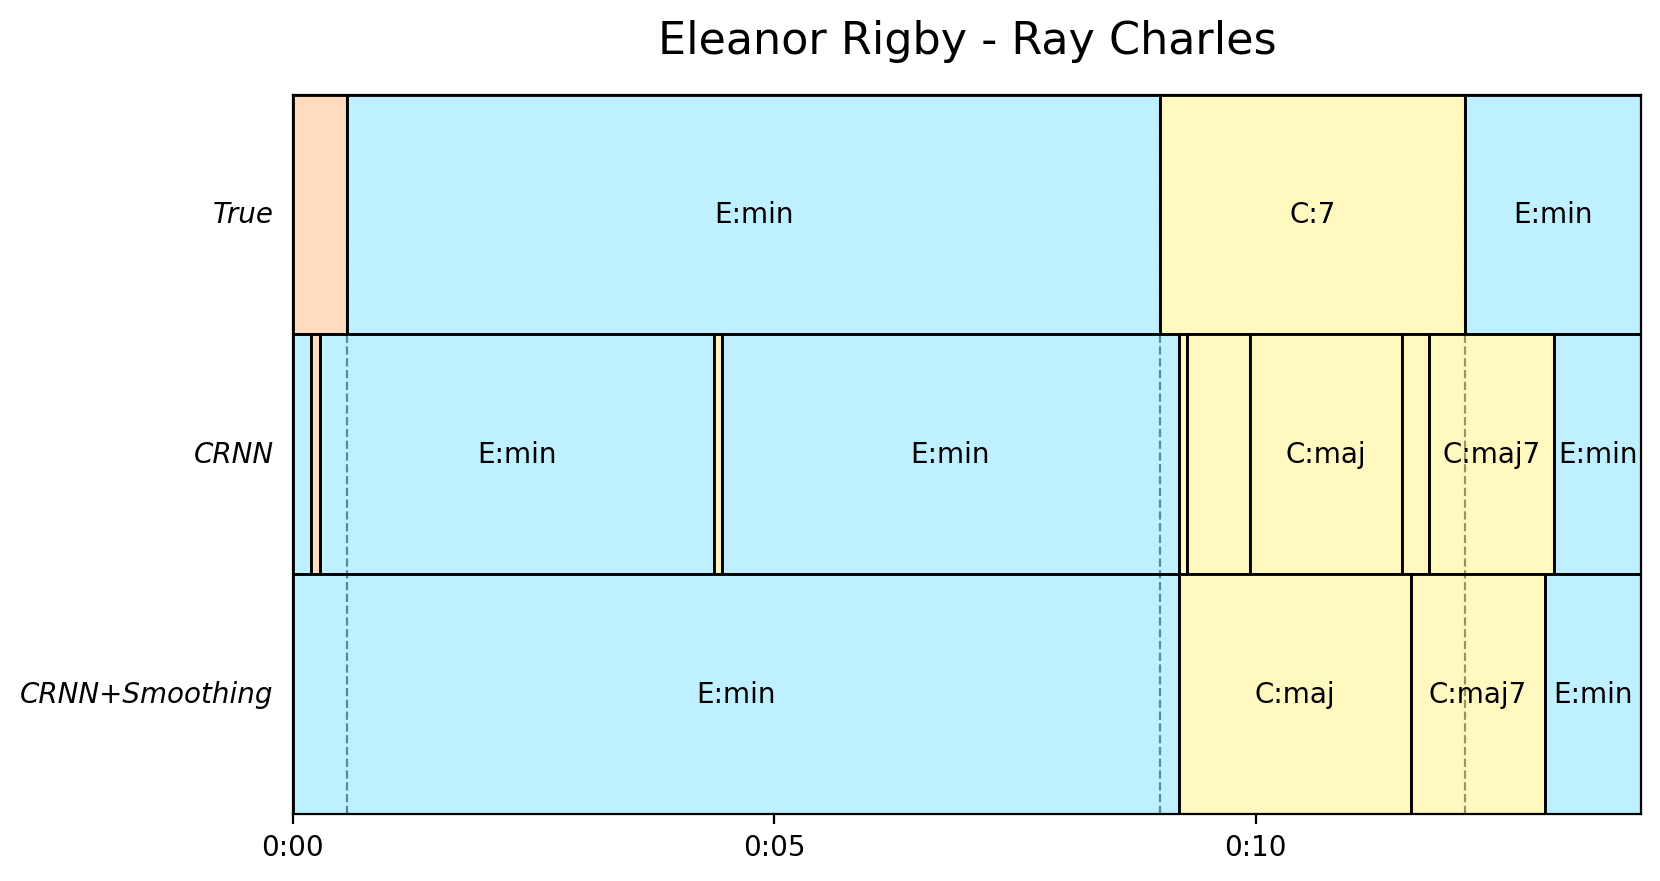
\includegraphics[width=0.9\textwidth]{figures/hmm_smoothing_example.png}
    \caption{An example of the effect of the HMM on the \emph{CRNN} model. The top plot shows the ground truth. The middle plot shows frame-wise predictions of the \emph{CRNN} without smoothing. The bottom plot shows the predictions after smoothing. Chords are coloured by their equivalent chord in the small vocabulary as it makes the plot easier to interpret. The original predictions contain many unnecessary and nonsensical chord transitions. These have been smoothed out by the HMM. The resulting chords appear more similar to the ground truth even if frame-wise accuracy has not changed much.}\label{fig:hmm_smoothing_example}
\end{figure}

We did not implement a CRF. All related works to use a CRF use a linear chain CRF with either hand-crafted transition penalties or learned transition penalties. We believe that such simple CRF's are unlikely to outperform the HMM given the effective smoothing of the HMM and do not explore further. We also do not wish to bias the model towards the transitions contained in the dataset. Given the long-tailed distribution, a learned transition matrix will further encourage the model to predict more common transitions. Thus, we believe that the HMM with a simple transition matrix which effectively smooths the predictions is a satisfactory solution.

\section{Pitch Augmentation}
- Two methods:
- On CQT \citet{ACRLargeVocab1}, not good.
- Using \texttt{pyrubberband}\footnote{\url{https://github.com/bmcfee/pyrubberband}} on the audio [everyone else], works?

Pitch augmentation has been done in other works on chord recognition. This has been done on the CQT~\citep{ACRLargeVocab1} by shifting the CQT bins and directly on the audio~\citep{BTC,StructuredTraining}. These are not the same process. Shifting the CQT is a simple matrix operation, whereas pitch shifting introduces other artefacts due to 

\section{Using Generative Features}

- As in [MelodyTranscriptionViaGenerativePreTraining], use Jukebox (?) to generate features at frames (? is it possible to do it on the same frames?). Train on these features and evaluate.


\section{Structured Training}

- Add structured loss and retrain. From literature. Should (?) further improve accuracies on sevenths etc.


\section{Synthetic Data Generation}\label{chap:synthetic_data}

Motivation

\subsection{Generation method} 
- Generation method. 
\subsection{Experiments}
- Brief description of the experiments and metrics I'm looking at
\subsection{Results}
- Results of the experiments on the validation set

\section{Results on the Test Set}

- Directly compare CRNN, weighted loss, pitch augmentation, structured, transformer, generative features, generated data and any meaningful combination on the test set.
- Also compare to BTC as a transformer model.

\subsection{Performance on JAAH}
- The performance of existing models on JAAH


\section{Qualitative Analysis}
- Qualitative analysis of the results